\documentclass[a0,landscape]{a0poster}

\usepackage[utf8]{inputenc}
\usepackage[T1]{fontenc}
\usepackage[scaled]{helvet}
\renewcommand{\familydefault}{\sfdefault}

\usepackage{graphicx}
\usepackage{xcolor}
\usepackage{tikz}
\usetikzlibrary{positioning, arrows.meta, fit, calc, matrix, backgrounds}

\usepackage[most]{tcolorbox}
\tcbuselibrary{skins}

\usepackage{array}

\usepackage[paperwidth=841mm, paperheight=1189mm,
  left=18mm, right=18mm, top=15mm, bottom=15mm,
  headheight=0pt, headsep=0pt, footskip=0pt]{geometry}

% ─── Colors (matching poster.html) ───
\definecolor{accBlue}{HTML}{2563EB}
\definecolor{accGreen}{HTML}{16A34A}
\definecolor{accRed}{HTML}{DC2626}
\definecolor{accOrange}{HTML}{EA580C}
\definecolor{accPurple}{HTML}{7C3AED}
\definecolor{accBlack}{HTML}{1A1A1A}
\definecolor{panelBg}{HTML}{F7F7F7}
\definecolor{quoteBg}{HTML}{E5E5E5}
\definecolor{bodyText}{HTML}{333333}
\definecolor{mutedText}{HTML}{666666}
\definecolor{highlightBg}{HTML}{FEF3C7}
\definecolor{h11light}{HTML}{5B9BFF}
\definecolor{h3light}{HTML}{4ADE80}
\definecolor{h14light}{HTML}{F87171}

\pagecolor{white}
\color{bodyText}

\setlength{\parskip}{0.2em}
\setlength{\parindent}{0pt}

% ─── Panel with a colored left accent bar ───
\newtcolorbox{qpanel}[1][accBlack]{%
  enhanced, arc=5mm,
  colback=panelBg, colframe=panelBg, boxrule=0pt,
  left=6mm, right=6mm, top=3mm, bottom=3mm,
  before skip=0mm, after skip=4mm,
  borderline west={3.5mm}{0mm}{#1},
}

\newcommand{\qtitle}[1]{{\Large\bfseries\color{accBlack}#1}\par\medskip}

\newtcolorbox{quotebox}{%
  enhanced, arc=3mm,
  colback=quoteBg, colframe=quoteBg, boxrule=0pt,
  left=5mm, right=5mm, top=3mm, bottom=3mm,
  before skip=3mm, after skip=3mm,
  fontupper=\itshape\color{bodyText}
}

\newcommand{\qlabel}[1]{{\normalfont\bfseries\color{accBlack}#1}}

\begin{document}
\thispagestyle{empty}
\noindent\begin{minipage}[t][\textheight][t]{\textwidth}

% ═══════════════════ TITLE BAR ═══════════════════
\begin{minipage}[b]{0.72\textwidth}
  {\veryHuge\bfseries Sixteen Voices}\\[5mm]
  {\huge\color{mutedText}A story of eight questions I asked a tiny transformer --- all on a laptop CPU}
\end{minipage}%
\hfill
\begin{minipage}[b]{0.26\textwidth}\raggedleft
  {\Huge\bfseries Katerina Fajmanova}\\[3mm]
  {\LARGE ML Prague 2026}\\[1mm]
  {\Large\color{mutedText}github.com/moudrkat/sixteen-voices}
\end{minipage}

\vspace{3mm}
{\color{accBlack}\rule{\textwidth}{3pt}}
\vspace{3mm}

% ─── SETUP STRIP ───
\noindent
\begin{tcolorbox}[enhanced, arc=4mm, colback=panelBg, colframe=panelBg, boxrule=0pt,
  left=6mm, right=6mm, top=3mm, bottom=3mm,
  borderline west={3mm}{0mm}{accBlack}]
  {\large
  \textbf{The setup.} I took TinyStories-1Layer-21M --- the smallest model that still writes coherent text (21M params, 1 layer, 16 heads) --- and fine-tuned it with \textbf{77 LoRA adapters}: 69 real authors from Project Gutenberg (Poe, Carroll, Grimm, Homer\ldots) plus 8 synthetic styles I designed myself to isolate one property each (minimalist, dialogue, questioner, cozy\ldots). Same prompt, different adapter, different voice. Then I spent months taking it apart.
  \par\smallskip
  \textbf{Prompt ``It was a dark and stormy''} $\rightarrow$
  \textcolor{accBlack}{\textbf{Poe:}} \textit{``the dark and sky wept. The dark sky above the clouds seemed to go away''} $\cdot$
  \textcolor{accBlack}{\textbf{Dialogue:}} \textit{``What do you know?'' asked the moon. ``I know sky,'' said the storm.}
  }
\end{tcolorbox}

\vspace{4mm}

% ═══════════════════ MAIN GRID ═══════════════════
\noindent
\begin{minipage}[t]{0.27\textwidth}

  % ═══ PART I banner ═══
  {\Large\bfseries\color{mutedText}Part I $\cdot$ Probing from the outside}\par
  \vspace{3mm}

  % ─── Q1 KNOCKOUT ───
  \begin{qpanel}[accBlue]
    \qtitle{Q1 $\cdot$ Do all 16 heads matter equally?}
    I knocked out each head across all 77 adapters --- one head at a time, zero the rest, measure how much of the style adaptation that single head recovers. That's \textbf{1,232 experiments}.

    Answer: no. \textbf{\color{accBlue}H11} dominates for 66\% of authors. \textbf{\color{accRed}H14} leads for a darker cluster --- Homer, Poe, Milton. They're \textbf{anticorrelated}: when one matters, the other doesn't.

    {\small\color{mutedText}Null check: untrained LoRA patches show \textbf{no specialization}. The pattern is learned, not architectural.\par}

    \vspace{3mm}
    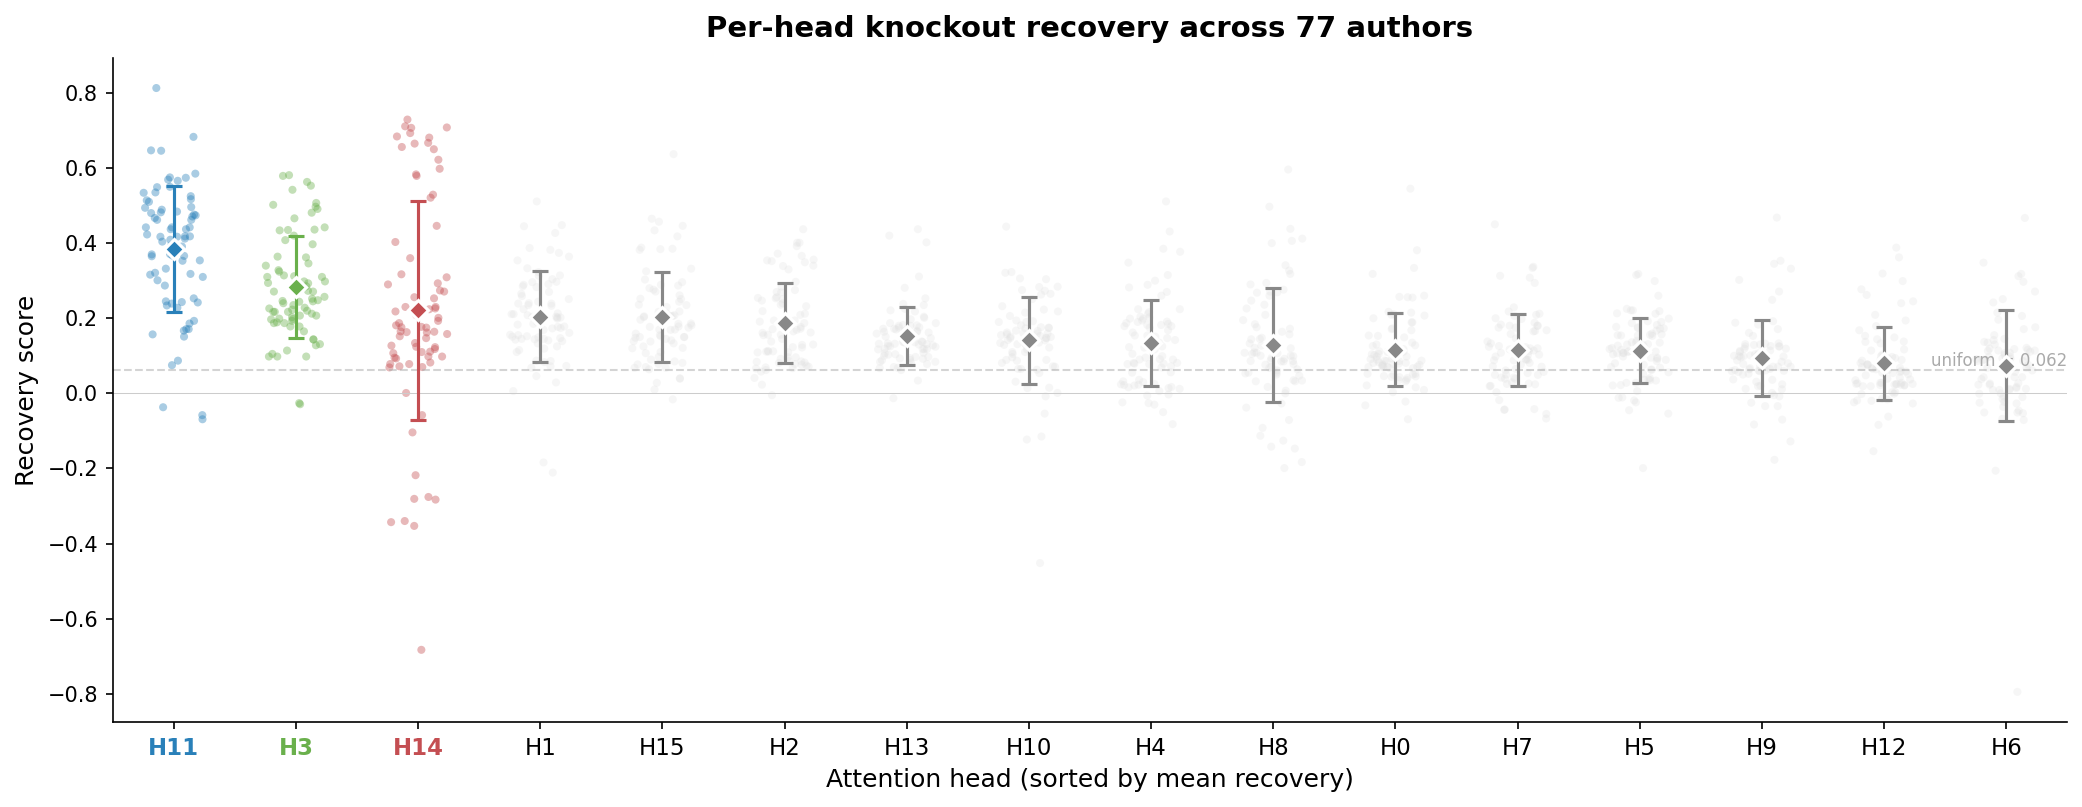
\includegraphics[width=\linewidth]{figures/knockout_strip_clean.png}
  \end{qpanel}

  % ─── Q2 STEER ───
  \begin{qpanel}[accBlue]
    \qtitle{Q2 $\cdot$ Can I steer a head like a dial?}
    Scale head outputs from 0$\times$ to 2$\times$ at inference time. Kill the dominant head $\rightarrow$ style vanishes.
    \textbf{Carroll without H11} = generic rabbit story. \textbf{Poe without H14} = nonsense.

    Unexpected finding along the way: LoRA changes \textbf{what} heads output, not \textbf{where} they look. Attention patterns are stable across all 77 adapters --- adaptation lives entirely in the value projections.

    \vspace{3mm}
    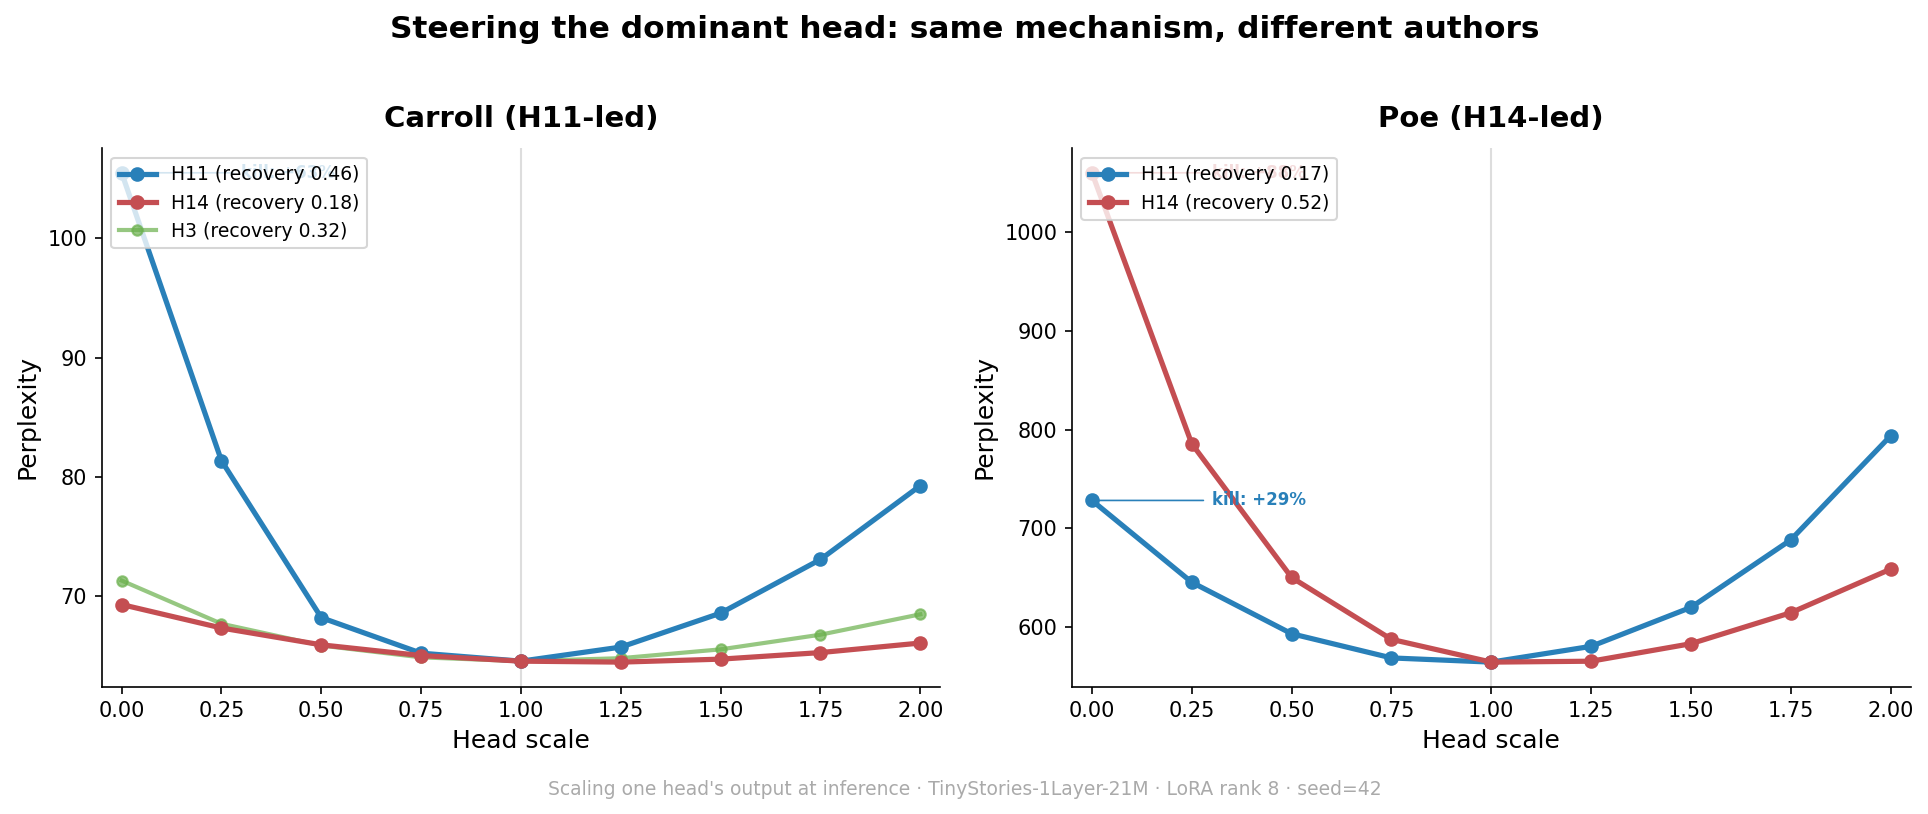
\includegraphics[width=\linewidth]{figures/steering_contrast.png}
  \end{qpanel}

  % ─── Q3 TRANSPLANT ───
  \begin{qpanel}[accPurple]
    \qtitle{Q3 $\cdot$ Can I transplant a head from one author to another?}
    Take Minimalist's adapter, replace just H14's weights with Poe's H14, generate. That's 64 out of 1024 weight rows --- 6\% of the LoRA.
    \begin{quotebox}
      \qlabel{Minimalist:} ``The trees began to tremble. The people were scared.''\\[1mm]
      \qlabel{+ Poe's H14:} ``Lightning flashed and thunder made me weep\ldots the thunder roared past her\ldots''
    \end{quotebox}
    The short sentence structure stays, Poe's dark vocabulary floods in. Works for Carroll and Grimm too.
  \end{qpanel}

  % ─── Q4 BLEND ───
  \begin{qpanel}[accBlack]
    \qtitle{Q4 $\cdot$ Can I blend two authors?}
    Linear interpolation: $(1{-}\alpha)\times$ Carroll $+ \alpha\times$ Poet.
    \begin{quotebox}
      $\alpha{=}0$: Alice asks questions inside the clouds.\\[1mm]
      $\alpha{=}0.5$: dialogue fades, the sky turns grey.\\[1mm]
      $\alpha{=}0.8$: line breaks appear between stanzas.\\[1mm]
      $\alpha{=}1$: full verse.
    \end{quotebox}
    \textbf{Smooth when adapters are close. Breaks when they're far apart} --- Poe $\rightarrow$ Carroll produces gibberish at the midpoint. LoRA weight space isn't a style space.
  \end{qpanel}

\end{minipage}%
\hfill
\begin{minipage}[t]{0.39\textwidth}

  % ─── CENTER: ARCHITECTURE ───
  \begin{tcolorbox}[enhanced, colback=white, colframe=accBlack,
    arc=6mm, boxrule=1.5pt,
    left=6mm, right=6mm, top=6mm, bottom=6mm]
    \centering
    \color{accBlack}
    {\Large\bfseries TinyStories-1Layer-21M}\\[1mm]
    {\small\itshape\color{mutedText}1 layer $\cdot$ 16 heads $\cdot$ 1024-dim residual $\cdot$ 50k vocab (GPT-Neo)}\\[6mm]

    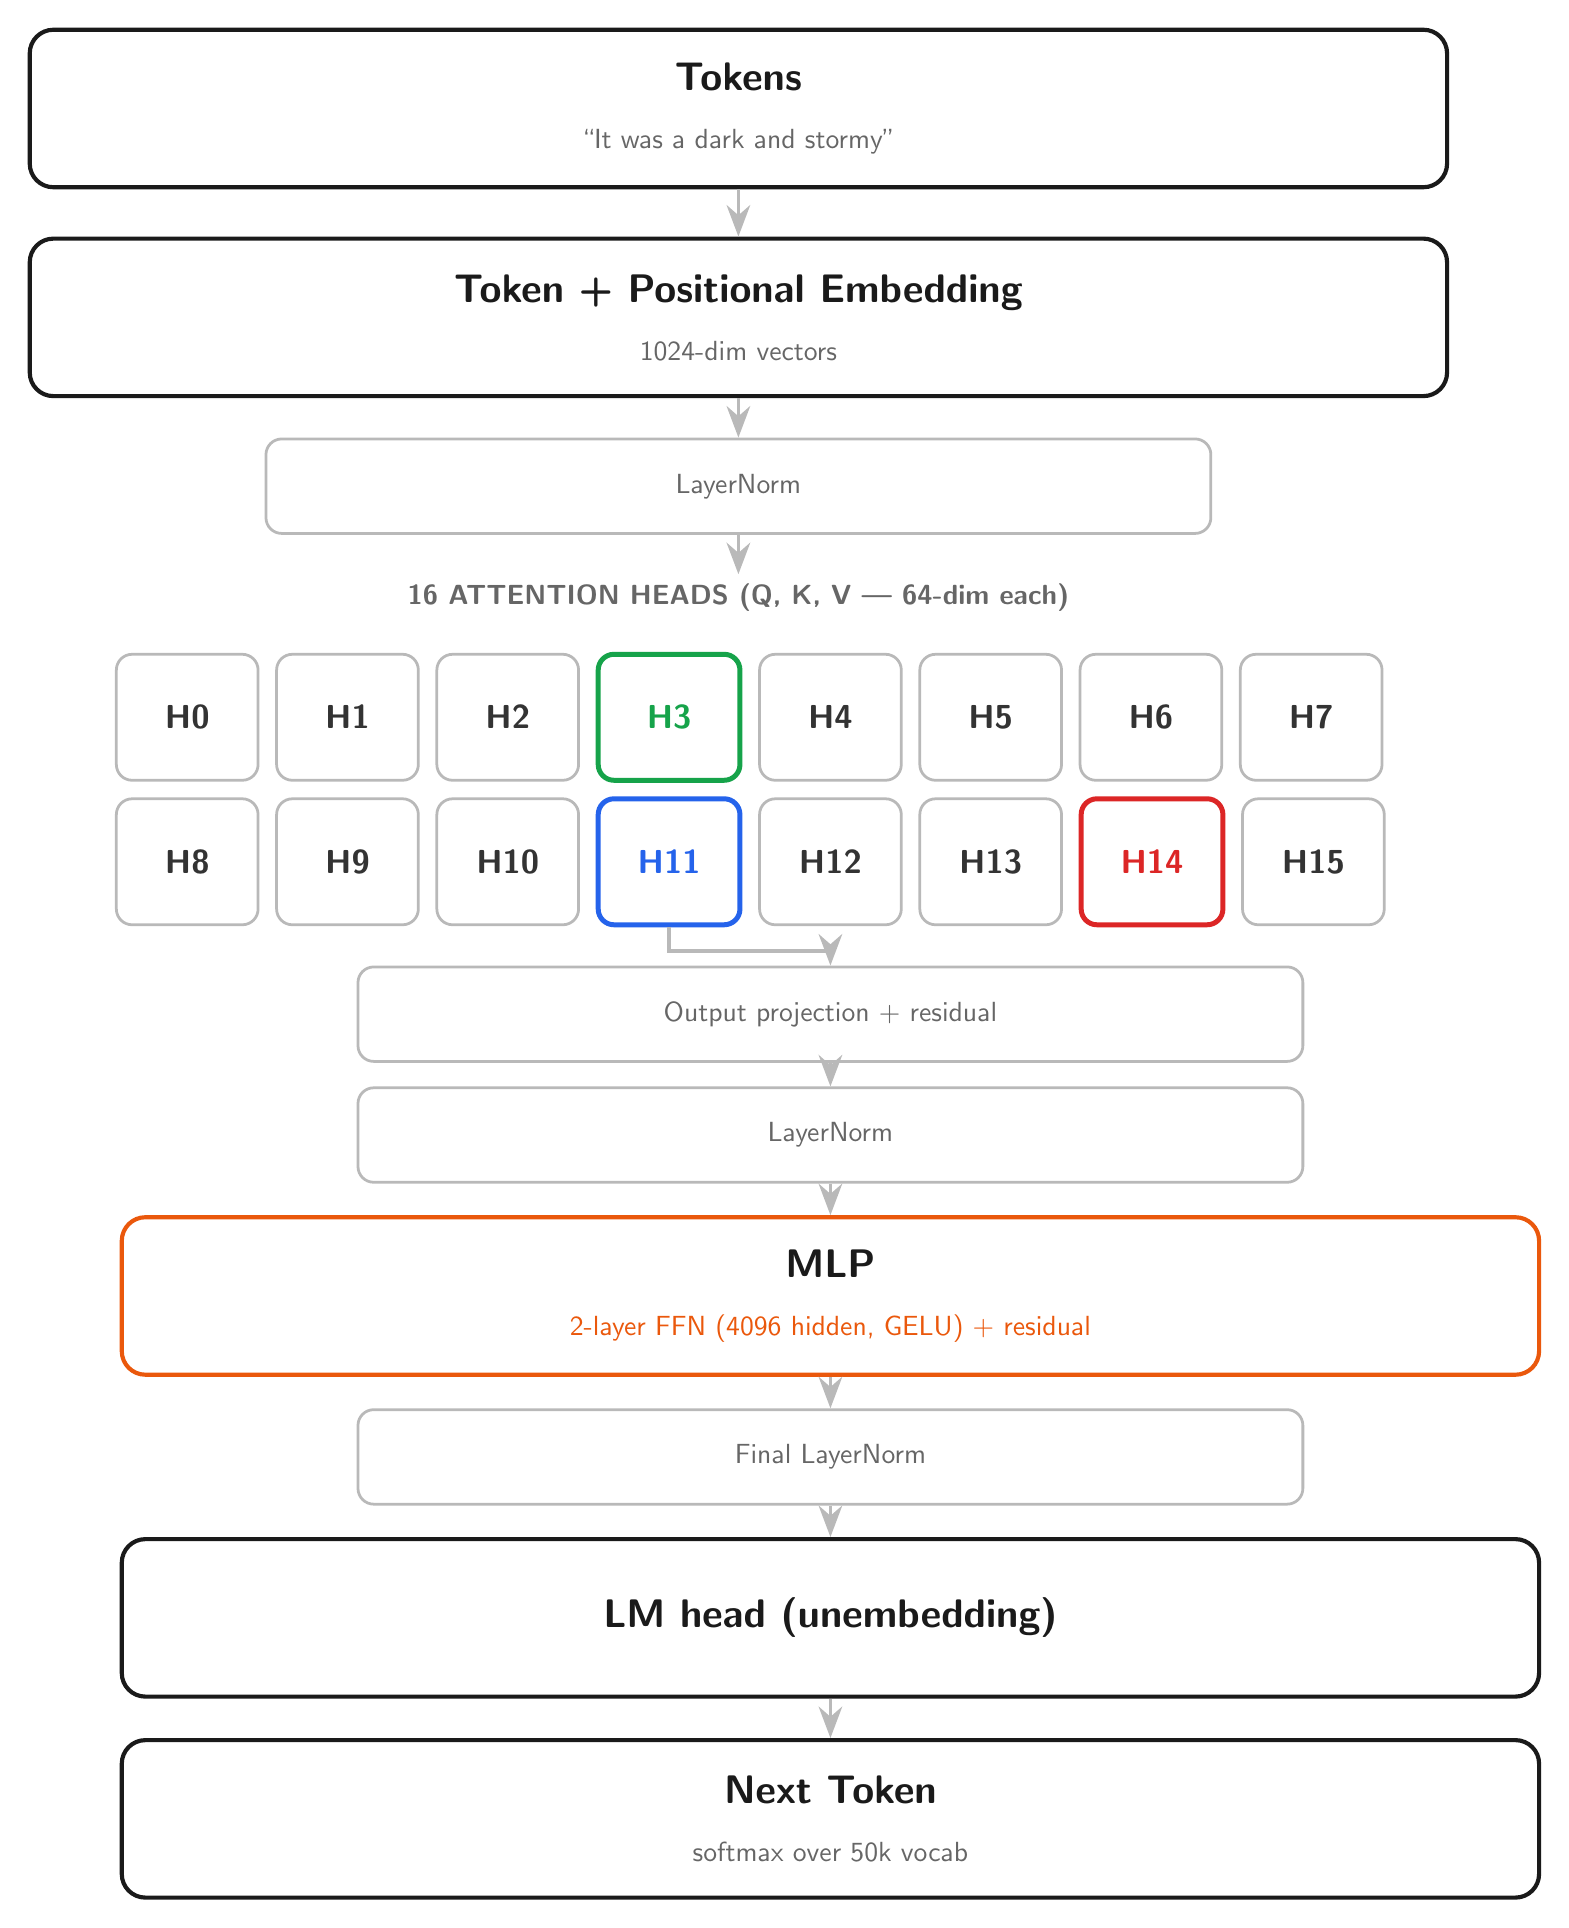
\begin{tikzpicture}[
      every node/.style={font=\Large},
      box/.style={rectangle, rounded corners=3mm, draw=accBlack, line width=1.5pt,
                  text=accBlack, minimum width=180mm, minimum height=20mm,
                  align=center, font=\Large\bfseries},
      lnbox/.style={rectangle, rounded corners=2mm, draw=gray!55, line width=1pt,
                    text=mutedText, minimum width=120mm, minimum height=12mm,
                    align=center, font=\normalsize},
      boxmlp/.style={box, draw=accOrange},
      head/.style={rectangle, rounded corners=2mm, draw=gray!55, line width=1pt,
                   text=bodyText, minimum width=18mm, minimum height=16mm, font=\large\bfseries},
      head11/.style={head, draw=accBlue, text=accBlue, line width=1.8pt},
      head3/.style={head, draw=accGreen, text=accGreen, line width=1.8pt},
      head14/.style={head, draw=accRed, text=accRed, line width=1.8pt},
      arr/.style={->, >={Stealth[length=4mm, width=3mm]}, gray!55, line width=1.2pt},
      sectlabel/.style={font=\normalsize\bfseries, color=mutedText},
    ]

      \node[box] (tokens) {Tokens\\[1mm]{\normalsize\color{mutedText}\normalfont``It was a dark and stormy''}};
      \node[box, below=6mm of tokens] (emb) {Token + Positional Embedding\\[1mm]{\normalsize\color{mutedText}\normalfont 1024-dim vectors}};
      \node[lnbox, below=5mm of emb] (ln1) {LayerNorm};

      % heads label + grid
      \node[sectlabel, below=5mm of ln1] (hlabel) {16 ATTENTION HEADS (Q, K, V --- 64-dim each)};

      % row 1: H0..H7
      \node[head, below=4mm of hlabel, xshift=-70mm] (h0) {H0};
      \node[head, right=2mm of h0] (h1) {H1};
      \node[head, right=2mm of h1] (h2) {H2};
      \node[head3, right=2mm of h2] (h3) {H3};
      \node[head, right=2mm of h3] (h4) {H4};
      \node[head, right=2mm of h4] (h5) {H5};
      \node[head, right=2mm of h5] (h6) {H6};
      \node[head, right=2mm of h6] (h7) {H7};

      % row 2: H8..H15
      \node[head, below=2mm of h0] (h8) {H8};
      \node[head, right=2mm of h8] (h9) {H9};
      \node[head, right=2mm of h9] (h10) {H10};
      \node[head11, right=2mm of h10] (h11) {H11};
      \node[head, right=2mm of h11] (h12) {H12};
      \node[head, right=2mm of h12] (h13) {H13};
      \node[head14, right=2mm of h13] (h14) {H14};
      \node[head, right=2mm of h14] (h15) {H15};

      % Output projection + residual add
      \node[lnbox, below=5mm of h12] (proj) {Output projection $+$ residual};
      \node[lnbox, below=3mm of proj] (ln2) {LayerNorm};
      \node[boxmlp, below=4mm of ln2] (mlp) {MLP\\[1mm]{\normalsize\color{accOrange}\normalfont 2-layer FFN (4096 hidden, GELU) $+$ residual}};
      \node[lnbox, below=4mm of mlp] (lnf) {Final LayerNorm};
      \node[box, below=4mm of lnf] (head) {LM head (unembedding)};
      \node[box, below=5mm of head] (out) {Next Token\\[1mm]{\normalsize\color{mutedText}\normalfont softmax over 50k vocab}};

      % arrows
      \draw[arr] (tokens) -- (emb);
      \draw[arr] (emb) -- (ln1);
      \draw[arr] (ln1) -- (hlabel);
      \draw[arr] (h11.south) -- ++(0,-3mm) -| (proj.north);
      \draw[arr] (proj) -- (ln2);
      \draw[arr] (ln2) -- (mlp);
      \draw[arr] (mlp) -- (lnf);
      \draw[arr] (lnf) -- (head);
      \draw[arr] (head) -- (out);

    \end{tikzpicture}

    \vspace{3mm}
    {\small\color{mutedText}\itshape H11 (blue) $\cdot$ H3 (green) $\cdot$ H14 (red) --- the heads that carry style}
  \end{tcolorbox}

  \vspace{6mm}

  % ─── REFS + QR ───
  \noindent
  \begin{minipage}[t]{0.70\linewidth}
    {\footnotesize\color{mutedText}
    {}[1] Eldan \& Li, ``TinyStories,'' 2023 \quad
    {}[2] Hu et al., ``LoRA,'' ICLR 2022 \quad
    {}[3] Michel et al., ``Are Sixteen Heads Really Better than One?'' NeurIPS 2019 \quad
    {}[4] Voita et al., ``Specialized Heads Do the Heavy Lifting,'' ACL 2019 \quad
    {}[5] Elhage et al., ``Transformer Circuits,'' Anthropic 2021 \quad
    {}[6] Turner et al., ``Activation Addition,'' 2023 \quad
    {}[7] Bricken et al., ``Towards Monosemanticity,'' Anthropic 2023 \quad
    {}[8] Templeton et al., ``Scaling Monosemanticity,'' Anthropic 2024 \quad
    {}[9] Ilharco et al., ``Task Arithmetic,'' ICLR 2023 \quad
    {}[10] Anthropic, ``Emotion Concepts,'' 2025
    \par}
  \end{minipage}%
  \hfill
  \begin{minipage}[t]{0.26\linewidth}\centering
    \fbox{\rule{0pt}{28mm}\rule{28mm}{0pt}}\\[1mm]
    {\scriptsize\color{mutedText}github.com/moudrkat/\\sixteen-voices}
  \end{minipage}

  \vspace{8mm}

  % ─── Q4 FIGURE: interpolation ───
  \begin{center}
    {\Large\bfseries\color{accBlack}Q4 $\cdot$ Blending Carroll $\rightarrow$ Poet}\par
    \vspace{1mm}
    {\small\color{mutedText}Linear interpolation between LoRA adapters. Dialogue fades, line breaks appear.}\par
    \vspace{2mm}
    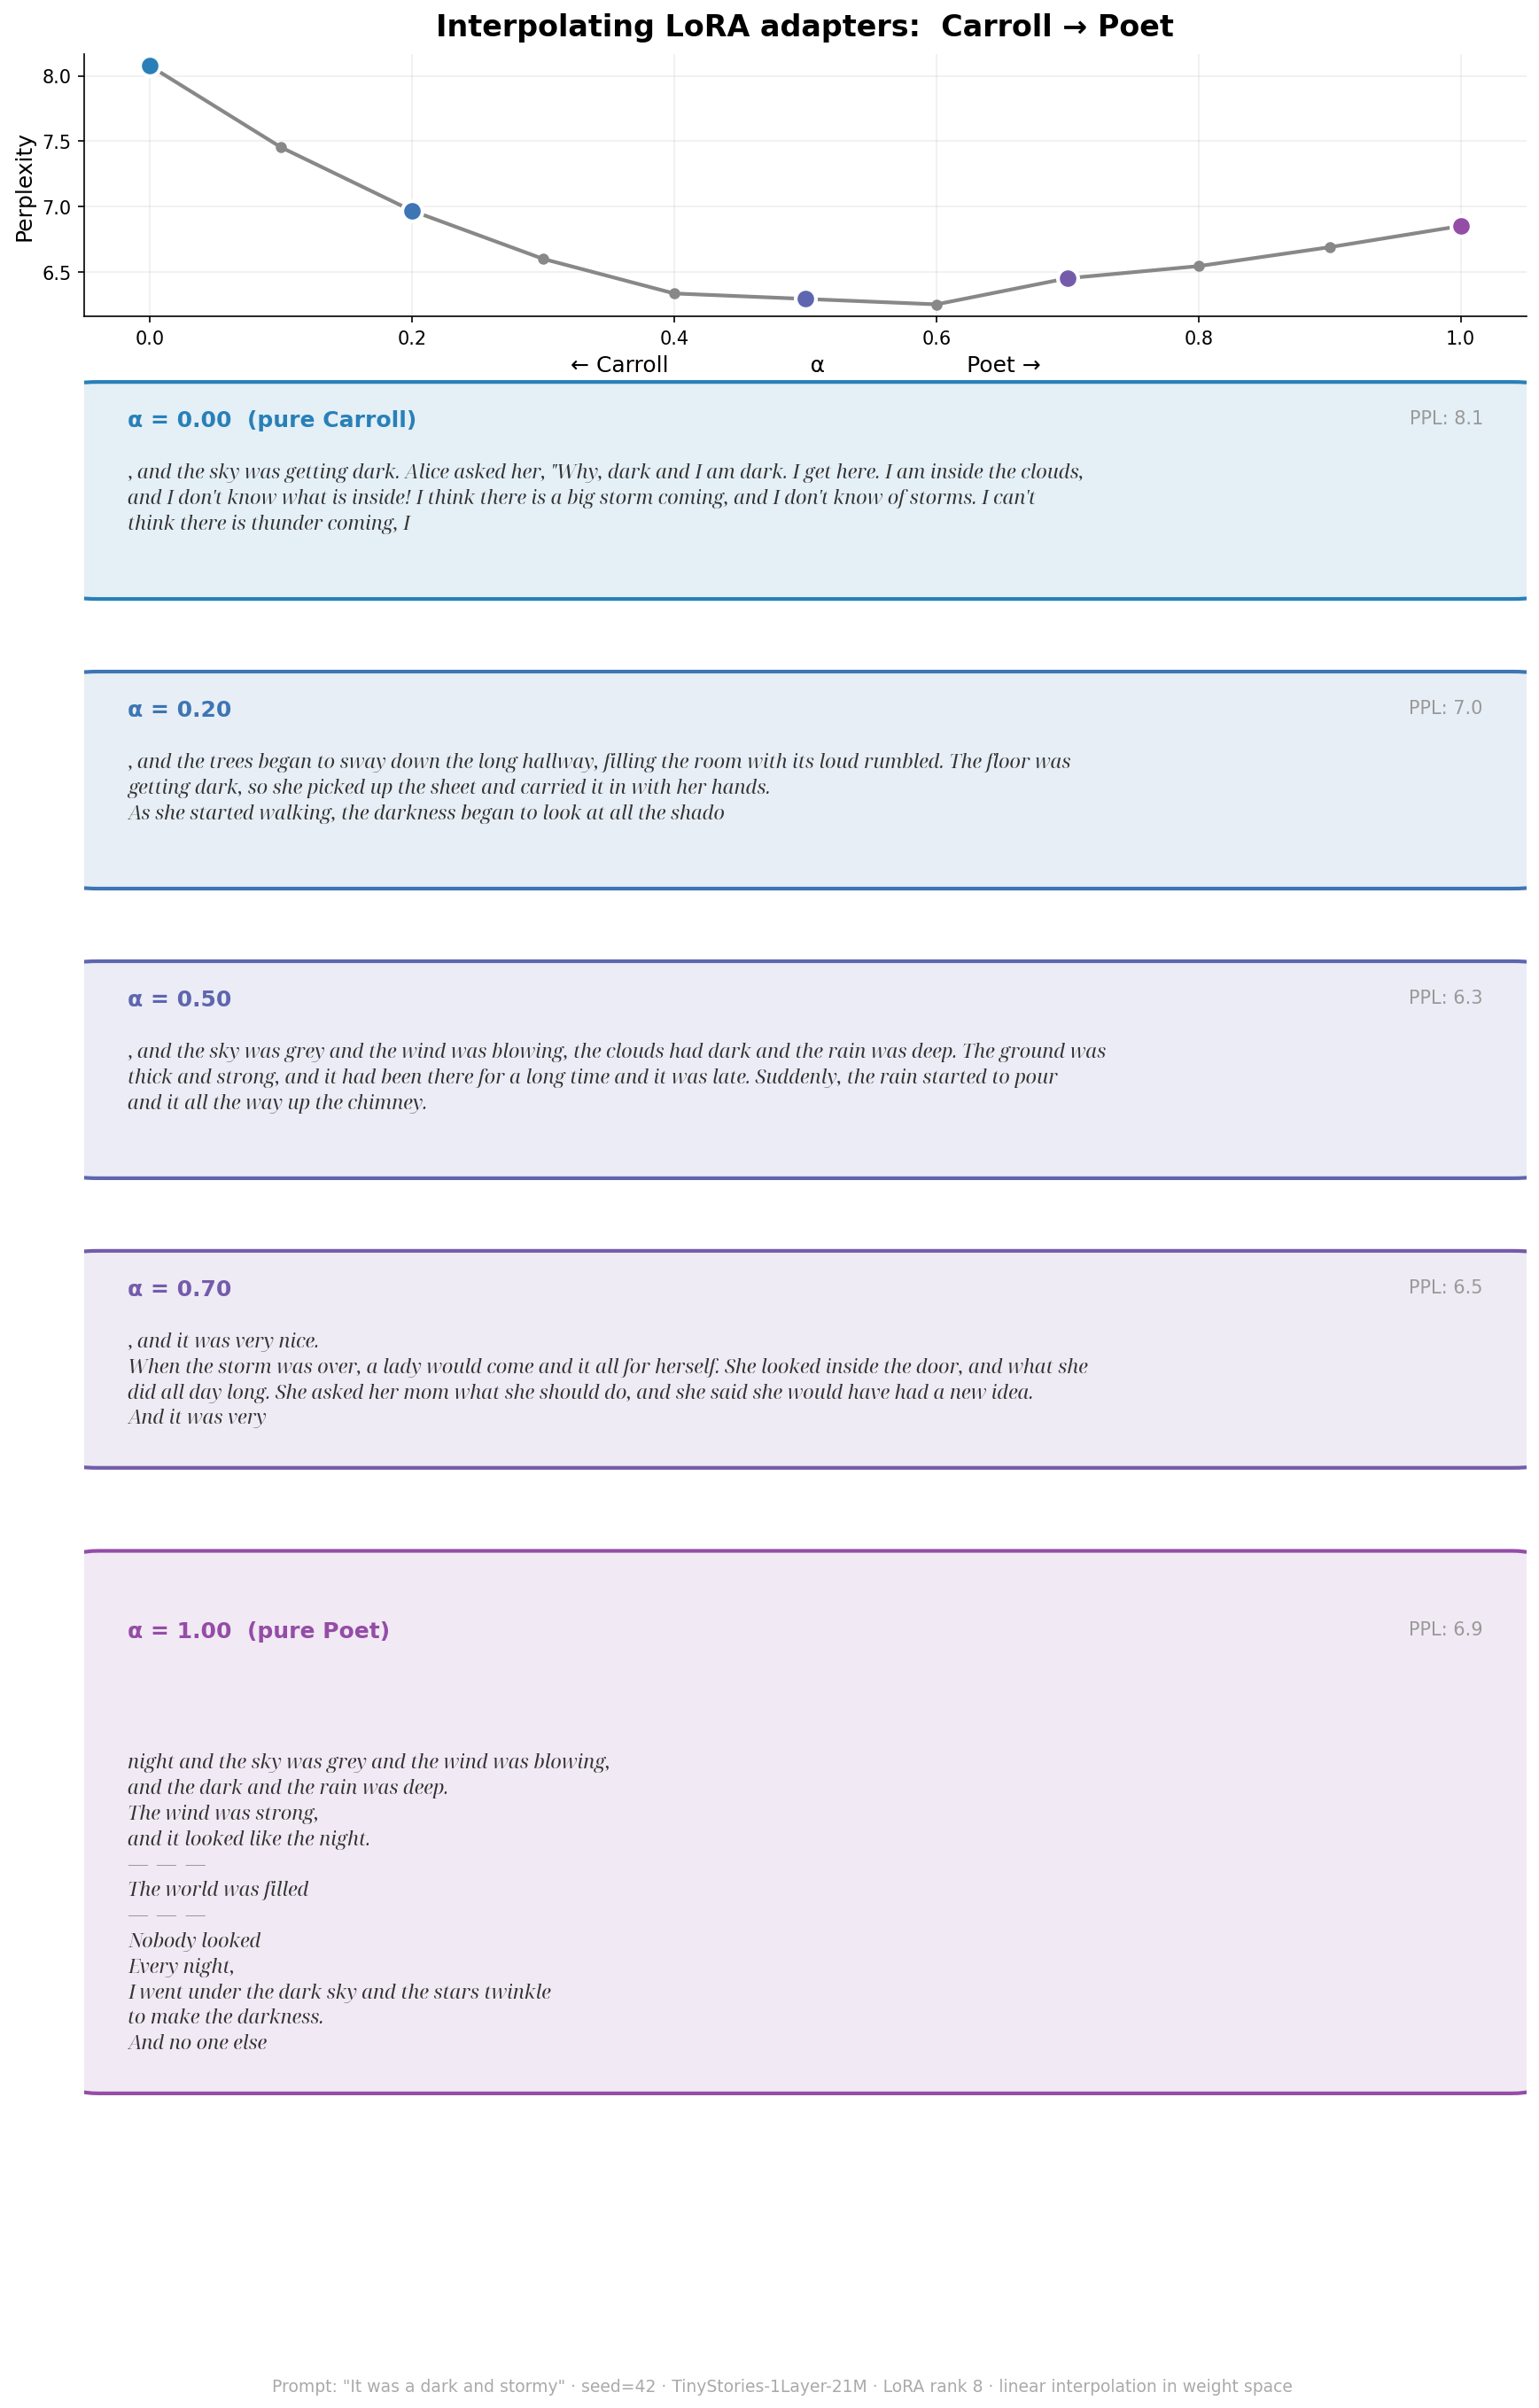
\includegraphics[width=0.92\linewidth, height=260mm, keepaspectratio]{figures/interpolation_linkedin.png}
  \end{center}

  \vspace{6mm}

  % ─── Q6 FIGURE: Carroll showcase ───
  \begin{center}
    {\Large\bfseries\color{accBlack}Q6 $\cdot$ Four feature knobs on Carroll's voice}\par
    \vspace{1mm}
    {\small\color{mutedText}Same prompt, same adapter, four SAE directions injected one at a time.}\par
    \vspace{2mm}
    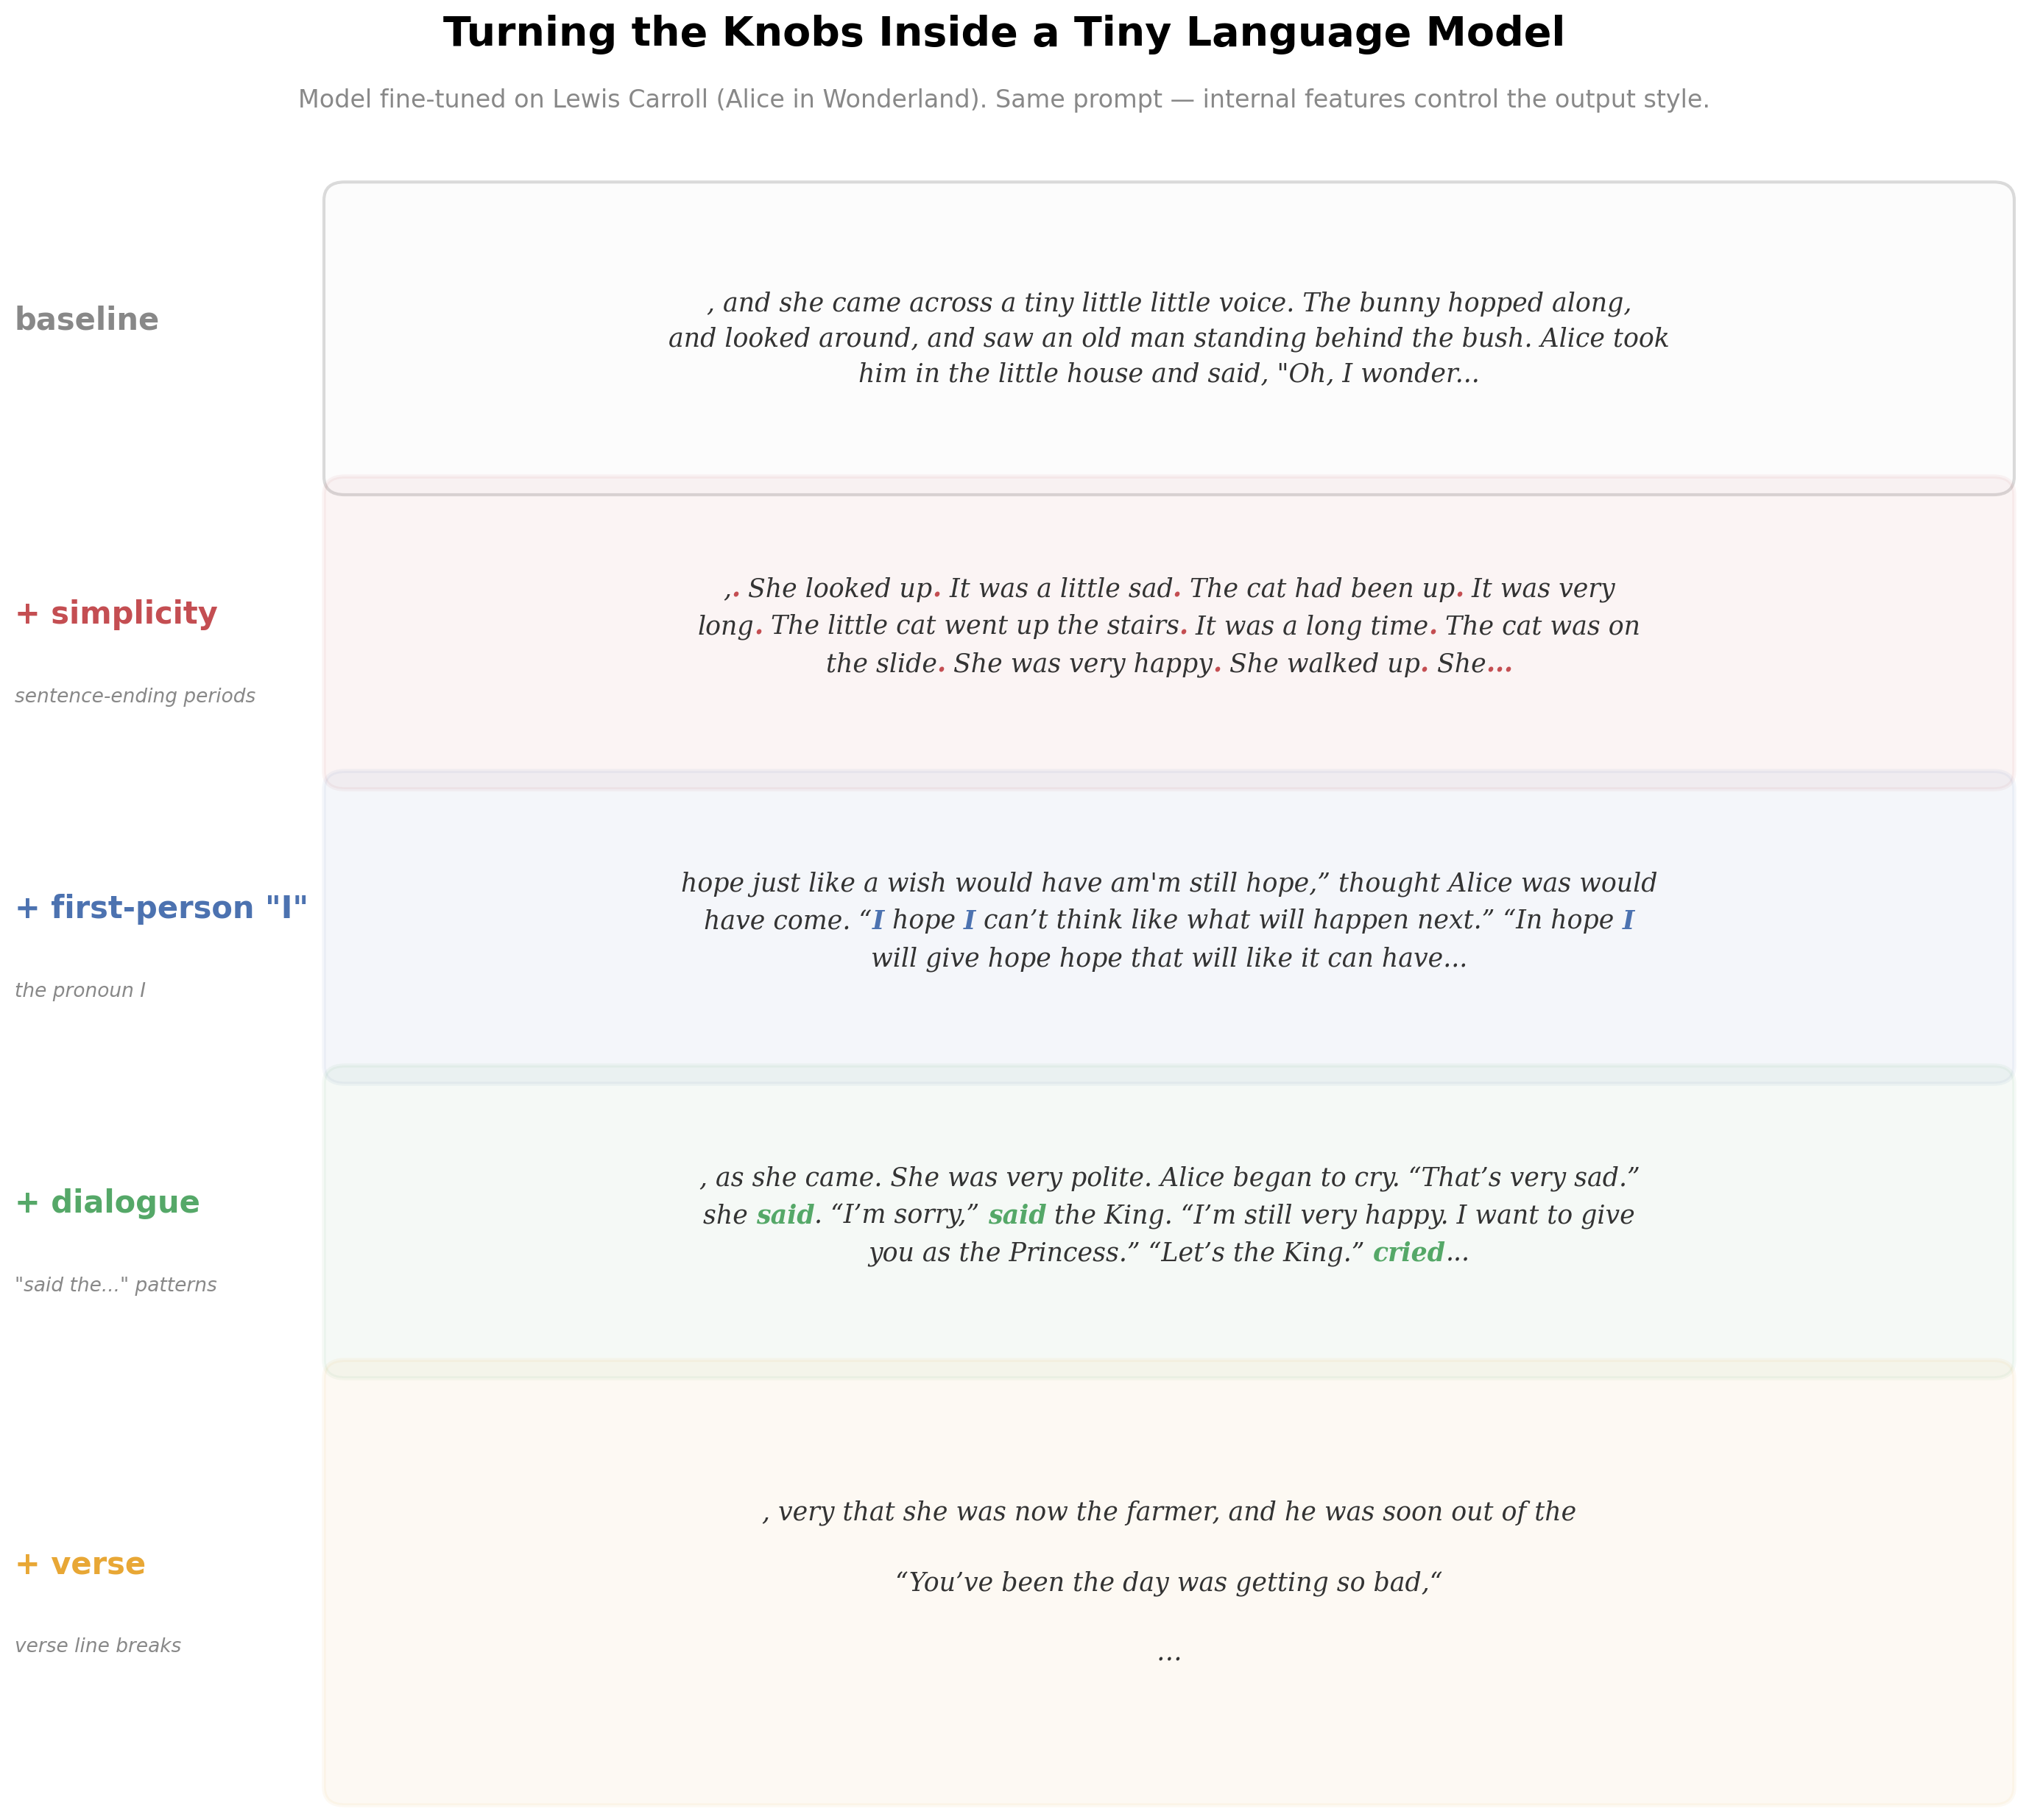
\includegraphics[width=0.92\linewidth, height=230mm, keepaspectratio]{figures/sae_showcase_carroll.png}
  \end{center}

\end{minipage}%
\hfill
\begin{minipage}[t]{0.27\textwidth}

  % ═══ PART II banner ═══
  {\Large\bfseries\color{mutedText}Part II $\cdot$ Looking inside}\par
  \vspace{3mm}

  % ─── Q5 SAE / HEAD ROLES ───
  \begin{qpanel}[accGreen]
    \qtitle{Q5 $\cdot$ What do these heads actually compute?}
    Knowing \emph{which} heads matter doesn't tell you \emph{what} they read. So I trained a \textbf{sparse autoencoder} on the residual stream --- 2048 features, 314 alive, $\sim$25 interpretable.

    Labels grounded: the synthetic controls were designed \textbf{before} the SAE existed, so each feature is cross-checked against a ground-truth author AND its top-activating tokens.

    {\color{accGreen}\textbf{H3}} --- swiss army knife, 107 features (reads all axes).
    {\color{accBlue}\textbf{H11}} --- opaque powerhouse: 17 features, zero overlap with any other head.
    {\color{accRed}\textbf{H14}} --- formality enforcer: suppresses ``I'', helps Homer (+0.73), hurts Shelley ($-$0.68).
    {\color{accOrange}\textbf{MLP}} --- 27 emergent features no head controls, including the strongest style direction.

    \vspace{2mm}
    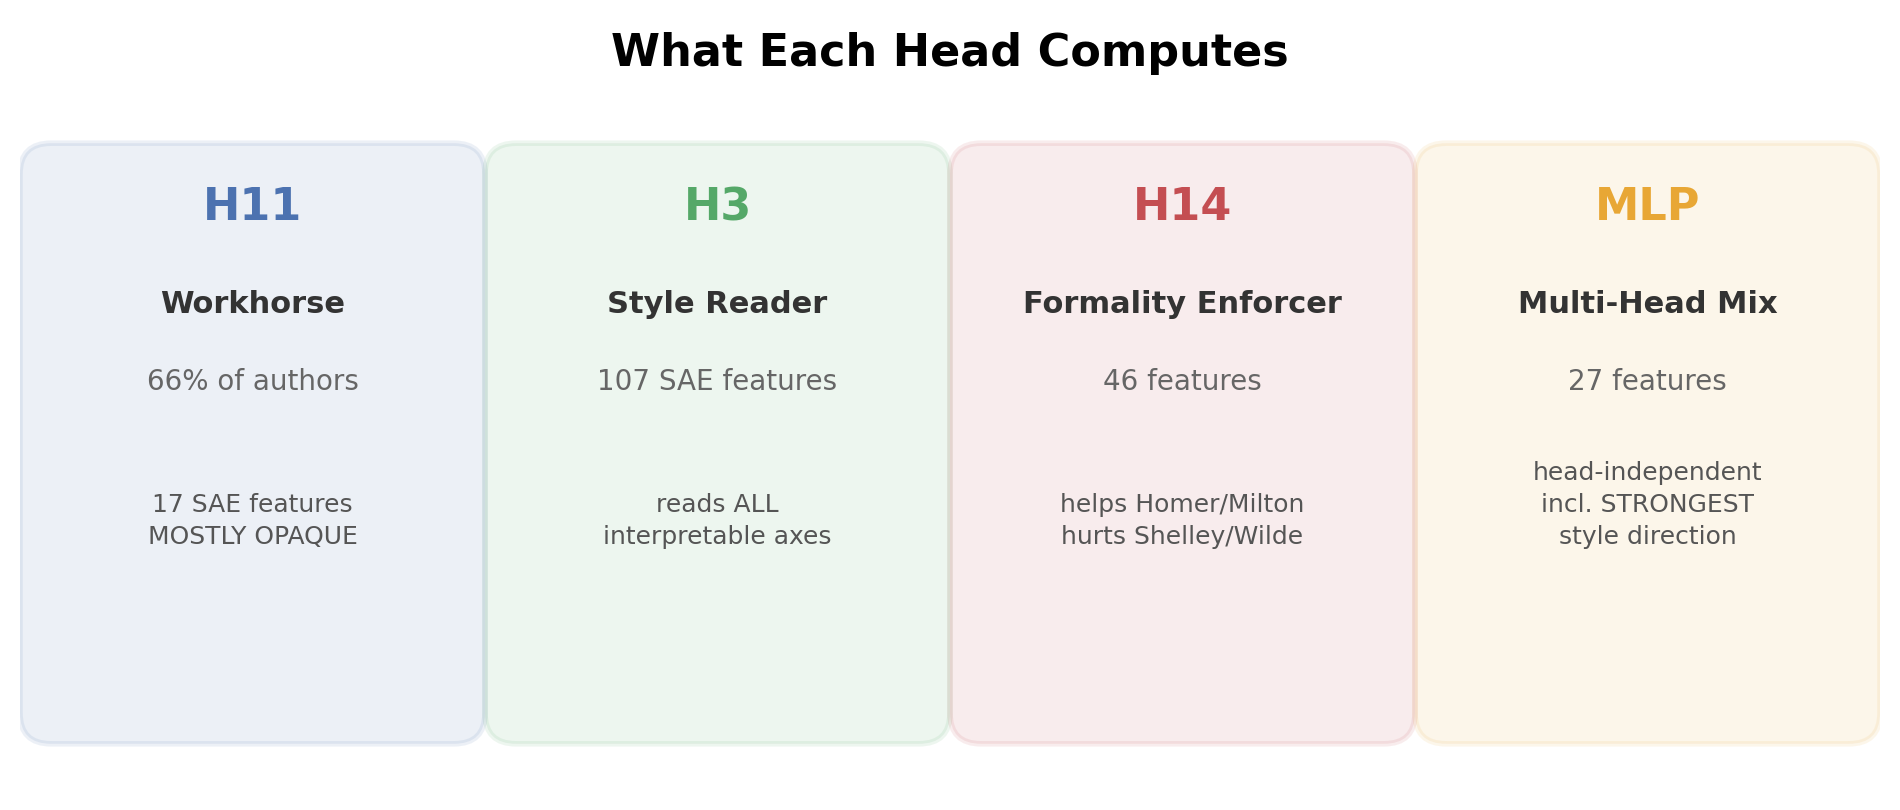
\includegraphics[width=\linewidth, height=70mm, keepaspectratio]{figures/poster_head_roles.png}
  \end{qpanel}

  % ─── Q6 FEATURE STEERING / COMPOSE ───
  \begin{qpanel}[accPurple]
    \qtitle{Q6 $\cdot$ Can I steer with individual features?}
    \textbf{Poe + simplicity:} gothic prose collapses to bare bones. Sentence length: 24 words $\rightarrow$ 5. 20/20 seeds.
    \begin{quotebox}
      \qlabel{Baseline:} ``the trees began to have to stop him from his bed. The dark and sky wept\ldots''\\[1mm]
      \qlabel{Steered:} ``It was dark. I went to sleep. It was dark. I woke up.''
    \end{quotebox}
    Features also \textbf{compose}. Base model + questions + dialogue + simplicity --- three subtle features, one new coherent voice:
    \begin{quotebox}
      \textit{``She asked her mommy, `Can I go outside and play?' Her mommy said, `Yes, but you must stay on the swing.'\,''}
    \end{quotebox}
  \end{qpanel}

  % ─── Q7 DETECTION ≠ STEERING ───
  \begin{qpanel}[accOrange]
    \qtitle{Q7 $\cdot$ Does detection equal steering?}
    \textbf{No.} Archaic-pronoun features fire perfectly on ``thou'' and ``thee'' in Blake and Milton. But injecting them produces nothing archaic --- the model degenerates first.
    \textbf{Perfect detectors, useless steering vectors.}

    Why? Compare with Anthropic's Golden Gate Bridge: Claude has billions of params and the bridge deep in its distribution. TinyStories has 21M. \textbf{Steering amplifies what the model can already express.}
  \end{qpanel}

  % ─── Q8 CONCLUSION ───
  \begin{qpanel}[accRed]
    \qtitle{Q8 $\cdot$ What did I find?}
    \colorbox{highlightBg}{\parbox{\dimexpr\linewidth-8mm}{\bfseries Style lives in two layers.}}

    \vspace{1mm}
    \textbf{STRUCTURAL} --- universal knobs (simplicity, dialogue, verse). Steer on any adapter.
    \textbf{SEMANTIC} --- author-specific fingerprints (dark atmosphere, cozy food, dialect). Detect everywhere. Steer only with the matching adapter.

    LoRAs \textbf{amplify}, they don't create. And the strongest style direction lives in the \textbf{MLP} --- invisible to any head.
  \end{qpanel}

\end{minipage}

\end{minipage}
\end{document}